\documentclass[11pt, oneside]{article}   	% use "amsart" instead of "article" for AMSLaTeX format
\usepackage{geometry}                		% See geometry.pdf to learn the layout options. There are lots.
\geometry{letterpaper}                   		% ... or a4paper or a5paper or ... 
%\geometry{landscape}                		% Activate for for rotated page geometry
%\usepackage[parfill]{parskip}    		% Activate to begin paragraphs with an empty line rather than an indent
\usepackage{graphicx}				% Use pdf, png, jpg, or eps� with pdflatex; use eps in DVI mode
								% TeX will automatically convert eps --> pdf in pdflatex		
\usepackage{amssymb}

\title{Gaussian Distribution (part 2)}
%\author{The Author}
\date{}							% Activate to display a given date or no date

\graphicspath{{/Users/telliott_admin/Dropbox/Tex/png/}}

\usepackage{listings,relsize} 
\lstloadlanguages{R} 
\lstset{language=R,basicstyle=\smaller[1],commentstyle=\rmfamily\smaller, 
  showstringspaces=false,% 
  xleftmargin=4ex,literate={<-}{{$\leftarrow$}}1 {~}{{$\sim$}}1} 
\lstset{escapeinside={(*}{*)}}   % for (*\ref{ }*) inside lstlistings (S code) 


\begin{document}

\maketitle
%\section{}
%\subsection{}
\large
\begin{center}
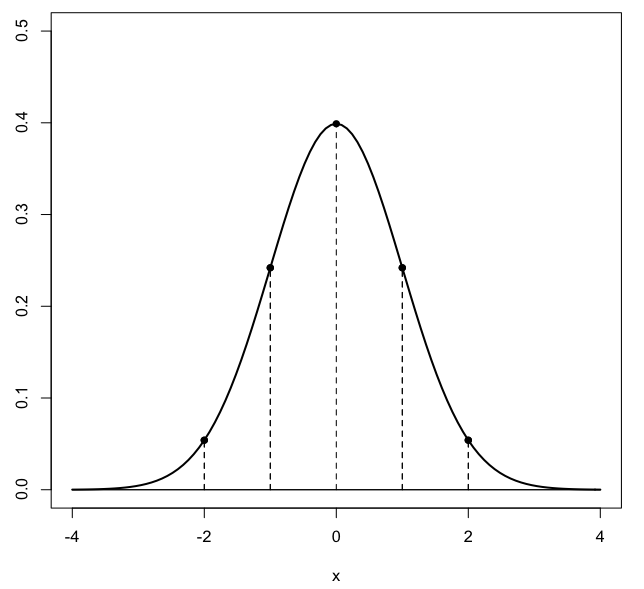
\includegraphics [scale=0.4] {gauss3.png}
\end{center}
The normal or Gaussian distribution, plotted above, is usually divided into sections according to $x = \pm n$ standard deviations.  It's an interesting fact that the first standard deviation corresponds to the inflection point of the curve.  At that point the second derivative of the function is equal to zero.

\[ G(x) = \frac{1}{\sigma \sqrt{2 \pi}} \ exp \ \{ \ -\frac{1}{2} (\frac{x - \mu}{\sigma} )^2\ \} \]
Let
\[ v(x) = -\frac{1}{2} (\frac{x - \mu}{\sigma} )^2 \]
\[ k = \sigma \sqrt{2 \pi} \]
\[ G(x) = \frac{1}{k} \ e^v \]

\[ G'(x) = \frac{1}{k} \  v' e^v\]
\[ \frac{dv}{dx} = -\frac{1}{\sigma} (\frac{x - \mu}{\sigma}) \]
\[ G'(x) = - \frac{1}{k} \  \frac{1}{\sigma} (\frac{x - \mu}{\sigma}) e^v\]

\[ G''(x) = \frac{1}{k} \ (-\frac{1}{\sigma}) (\frac{x - \mu}{\sigma}) (-\frac{1}{\sigma}) (\frac{x - \mu}{\sigma}) e^v + k (\frac{1}{\sigma}) e^v \]
\[ G''(x) = \frac{1}{k} \ (\frac{1}{\sigma^2}) \ [(\frac{x - \mu}{\sigma})^2 - 1] \ e^v \]
We want
\[ G''(x) = 0 \]
where
\[ e^v = exp \ \{ \ -\frac{1}{2} (\frac{x - \mu}{\sigma} )^2\ \} \]
In the limit as $x \to \pm \infty$, the term above approaches $0$, but those are not the solutions we want.  So we need
\[ (\frac{x - \mu}{\sigma})^2 - 1 = 0 \]
\[ (x-\mu)^2 = \sigma^2 \]
\[ x = \mu \pm \sigma \]
The second derivative required some bookkeeping, but was simple in the end.

What about the constant in front?  It's there to make the sum of the area under the probability distribution, the cumulative distribution function, equal $1$.  There is no way to solve the integral, it must be computed numerically.  If you do that for $e^v$ as defined above (no leading constant $\frac{1}{k} \ $), you find that the value is $k$.  So this is a "normalizing constant", to make the whole thing equal to $1$.

I have some notes about how to find a value for this integral.  What we will show is that
\[ \int_{-\infty}^{+\infty} \ e^{-x^2} \ dx = \sqrt{\pi} \]
Rather than use $-x^2$ do
\[ \int \int e^{-(x^2 + y^2)} \ dx \ dy \]
Since
\[ e^{-(x^2 + y^2)} = e^{-x^2} e^{-y^2} \]
this is 
\[ [ \ \int e^{-x^2} dx \ ]^2 \]
by iterated integrals.  Now switch to polar coordinates
\[ \int \ \int e^{-r^2} r \ dr \ d\theta \]
\[ 0 <= \theta <= 2 \pi \]
\[0 <= r <= \infty \]
Rather than use $\infty$ (this is an improper integral) use $a$ (very large).  The inner integral is \[ -\frac{1}{2} e^{-r^2}  \bigg |_0^a = \frac{1}{2} (1- e^{-a^2}) \]
The outer integral is just $2\pi$, so we have
\[ (2\pi) \ \frac{1}{2} (1- e^{-a^2}) \]
As $a \to \infty$, this $\to \pi$.
Here is a second way:
\[ \int_{-\infty}^{\infty}\ \int_{-\infty}^{\infty} \ e^{-(x^2 + y^2)} \ dy \ dx = 4 \int_{0}^{\infty}\int_{0}^{\infty} \ e^{-(x^2 + y^2)} \ dy \ dx \]
Substitute (remember the extra $4$ for later)
\[ y = xs, dy = x ds \]
\[ \int_{0}^{\infty} \ [ \ \int_{0}^{\infty} \ e^{-x^2(1 + s^2)} x \ ds \ ] \ dx \] 
\[ \int_{0}^{\infty} \ [ \ \int_{0}^{\infty} \ e^{-x^2(1 + s^2)} x \ dx \ ] \ ds \] 
The inner integral is
\[ -\frac{1}{2(1+s^2)} e^{-x^2(1+s^2)} \ \bigg |_0^\infty = (\frac{1}{2}) \frac{1}{1+s^2} \]
The outer integral is
\[
\int_0^\infty \ (\frac{1}{2}) \frac{1}{1+s^2} \ ds = \frac{1}{2} arctan(s) \ \bigg |_0^\infty = \frac{\pi}{4} \]
Pick up the $4$ from the beginning and we have just $\pi$.
The general result is that
\[ \int_{-\infty}^{+\infty} \ e^{-(x+b)^2/c^2} \ dx = c \sqrt{\pi} \]


\subsection*{R code}
\begin{lstlisting}
plot(dnorm,xlim=c(-4,4),ylim=c(0,0.5),lwd=2)
X = c(-2,-1,0,1,2)
Y = dnorm(X)
points(X,Y,pch=16)
for (i in 1:length(X)) {
    lines(c(X[i],X[i]),c(0,Y[i]),lty=2) }
lines(c(-4,4),c(0,0))
\end{lstlisting}

\end{document}  